\newpage

\section{Минимальные $k$-связные графы}

\subsection{Расцепление пары зависимых нормальных разрезов (Леммы 4 и 5).}

В данной главе по умолчанию считаем что граф $G$ ~--  $k$-связный. \todo[inline]{но не обязательно минимальный?}

\begin{df*}[Критическое ребро]
	Назовем ребро $e \in E(G)$ $k$-связного графа  $G$ критическим, если граф  $G - e$ не является  $k$-связным.
\end{df*}

\begin{df*}[Минимальный граф]
	Назовем $k$-связный граф минимальным, если все его ребра - критические.
\end{df*}

\begin{prop} \label{prop:for_minimum_k_connected_graph}
	Для минимального $k$ связного графа  $G$ обозначим:
	 \begin{itemize}
		 \item $V_k$ - множество вершин степени ровно  $k$
		 \item  $V_{k +1}$ - множество вершин степени хотя бы  $k + 1$. 
		 \item $v_k = |V_k|, v_{k + 1} = |V_{k + 1}|$
		 \item  $G_{k+1} = G(V_{k + 1}), E_{k + 1} = E(G_{k + 1})$
		\item  $e_k$ - количество ребер между вершинами степени  $k$
		\item $c$ - количество компонент связности графа  $G_{k + 1}$
		\item Для каждого ребра  $e \in E(G)$ существует разрез, содержащий  $e$ и  $k - 1$ вершину, в силу минимальности $G$. Более того, это ребро не инцидентное ни одной вершине множества.
			Обозначим множество всех таких разрезов за  $\R$.
	\end{itemize}

	Вершин кроме $V_k$ и  $V_{k+1}$ в графе  $G$ нет, т.к. он  $k$-связный.
\end{prop}

Напомним, что тогда $|\Part(S) = 2|, \forall S \in \R$, ведь при возвращении ребра  $e$ граф опять становится связным.

\begin{customlm}{3.1}[W.Mader.] \label{lemma:3_1}
	Пусть $G$ -  $k$-связный граф,  $a, b, c \in V_{k + 1}(G)$, ребра  $ab, ac \in E(G)$ - критические, а разрезы  $T, S \in \R$ таковы, что $ab \in T, ac \in S$.
	Пусть  $\Part(T) = \{H_a, \overline H_a\}$,  $\Part(S) = \{F_a, \overline F_a\}$, где  $a \in H_a$ и  $a \in F_a$.
		Тогда  $|H_a| > |\overline F_a|$.
\end{customlm}

\begin{proof}
	Док-во входит в другой курс, поэтому тут не обсуждается :)

	В билеты входить не будет(вроде бы).

	% Аналогично у следующих двух утверждений.
\end{proof}

\begin{customthm}{3.0}[W.Mader, 1972] \label{theorem:3_0}
	Пусть $G$ - минимальный  $k$-связный граф.
	Тогда  $G_{k + 1}$ ~-- лес.
\end{customthm}

% \begin{crly*}[W. Mader, 1972]
% 	Пусть $G$ - минимальный  $k$-связный граф.
% 	Тогда 
% 	 \[
% 		v_k(G) \geqslant \frac{(k - 1) \cdot v(G) + 2}{2k - 1}
% 	\] 
% \end{crly*}

% В 1979 Мадер доказал более сильное утверждение:

\begin{customthm}{3.1}[W.Mader, 1979] \label{theorem:3_1}
	Для минимального $k$ связного графа  $G$ выполнено:

	\[
		v_k(G) \geqslant \frac{(k - 1) \cdot v(G) + 2k}{2k - 1}
	\] 

\end{customthm}

Эта оценка точная: для любого $k \geqslant 2$ существуют бесконечные серии минимальных  $k$-связных графов, на которых она обращается в равенство.

\begin{df*}[Экстремальных минимальный $k$-связный граф]
	Будем называть минимальный $k$-связный граф \textbf{экстремальным}, если 

	 \[
		v_k(G) = \frac{(k - 1) \cdot v(G) + 2k}{2k - 1}
	\] 
\end{df*}

\begin{prop*}[$\triangle$]
	Для произвольного графа  $G$ обозначим  $\triangle(G)$ - максимальную степень вершины в  $G$.
\end{prop*}

\begin{df*}[$G_{k,T}$]
	Пусть $T$ - дерево с  $\triangle(T) \leqslant k + 1$ и $k \geqslant 2$.
	Граф $G_{k, T}$ строится из  $k$ копий  $T_1, \ldots, T_k$ дерева $T$.
	Для каждой вершины  $a \in V(T)$ обозначим  $a_i$ - соответствующую копию вершины в $T_i$.
	Если  $\deg_G(a) = j$, то ты добавим  $k + 1 - j$ новых вершин степени  $k$, смежных с  $\{a_1, \ldots, a_k\}$

\begin{figure}[ht]
    \centering
	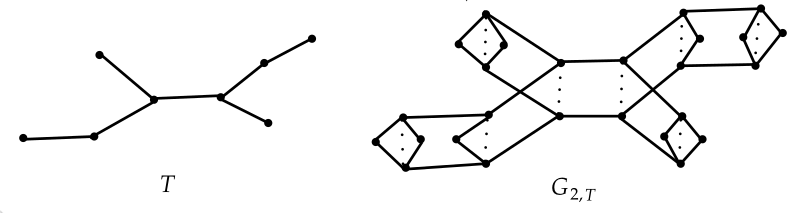
\includegraphics[width=0.5\columnwidth]{figures/3_definition_g_k_t.png}
    \caption{Рисунок к определению $G_{k, T}$}
\end{figure}

	Тогда очевидно, что если $|V(T)| = n$, то:

	\begin{align*}
		v(G_{k, T}) = kn + \sum_{a \in V(T)} (k + 1 - \deg_T(a)) &= kn + (k + 1)n - 2 (n - 1) =\\
																&=(2k - 1)n + 2
	\end{align*}

	Несложно проверить, что  $G_{k, T}$ - минимальный $k$-связный граф. 

	Экстремальность:

	\begin{align*}
		v_k(G_{k, T}) = \sum_{a \in V(T)} (k + 1 - \deg_T(a)) = (k + 1)n - 2(n - 1) &= (k - 1)n + 2 \\
		\frac{(k - 1) \cdot ((2k - 1)n + 2) + 2k}{2k - 1} &= (k - 1) n + 2
	\end{align*}


\end{df*}

\begin{customthm}{3.2} \label{theorem:3_2}
	Любой экстремальный минимальный $k$-связный граф - это граф  $G_{k, T}$ для некоторого дерева  $T$ с  $\triangle(T) \leqslant k + 1$.
\end{customthm}


\begin{prop*}
	Пусть разрезы $S, T \in \R$ зависимы, причем входящие в них ребра различны(но могут иметь общий конец).
	Обозначим $\Part(S) = \{F_1, F_2\}, \Part(T) = \{H_1, H_2\}$
	Введем обозначения:

	\begin{itemize}
		\item $G_{i,j} = F_i \cap H_j$, $P = T \cap S$
		\item  $T_i = \Int(F_i) \cap T, \ S_j = \Int(H_j) \cap S$
		\item $\Int(G_{i, j}) = G_{i, j} \setminus (P \cup T_i \cup S_j)$
		\item Пусть  $R_{i, j} = \Cut(G_{i, j})$, где $\Cut(G_{i, j})$ - граничный разрез части  $G_{i, j}$, а именно объединение  $\Bound(G_{i, j})$ и ребер  $S, T$, которые инцидентные вершинам  $\Int(G_{i, j})$.
		\item $\overline G_{i, j}$ - объединение трёх отличных от  $G_{i, j}$ частей.
	\end{itemize}

	Множество $P$ в нашем случае содержит только вершины.

\end{prop*}

\begin{figure}[ht]
    \centering
	\incfig[0.2]{prop_dependent_cuts_k_connected_graph}
	\caption{$\Cut(G_{1, 2})$ это объединение красных ребер и области заштрихованной зеленым}
    \label{fig:prop_dependent_cuts_k_connected_graph}
\end{figure}

\begin{customlm}{3.2} \label{lemma:3_2}
	$|R_{i, j}| + |R_{3 - i, 3 - j}| \leqslant |S| + |T| = 2k$
\end{customlm}

\begin{proof}
	Множество $R_{i, j}$ состоит из  $P \cup T_i \cup S_j$ и ребер разрезов  $T$ и  $S$, инцидентных вершинам из  $\Int(G_{i, j})$.

	Вершины из $P$ в обеих частях считаются дважды, а остальные вершины и рёбра из  $S$ и  $T$ в левой части считаются не более чем один раз, а в правой части - ровно один раз.
\end{proof}

\begin{customlm}{3.3} \label{lemma:3_3}
	Пусть $c$ - количество компонент связности графа  $G_{k + 1}$, тогда

	\[
		v_k(G) \geqslant \frac{(k - 1)|V(G)| + 2(c + e_k)}{2k - 1}
	\] 

	причем равенство может достигаться только при $\triangle (G) \leqslant k + 1$

\end{customlm}

\begin{proof}
	Из каждой вершины множества $V_{k + 1}$ выходит не менее  $k + 1$ ребра.
Сумма степеней леса  $G_{k + 1}$ равна  $2v_{k + 1} - 2c$, следовательно, не менее чем  $(k - 1) v_{k + 1} + 2c$ ребер выходит из $V_{k +1}$ в  $V_k$.

Из вершин множества $V_k$ выходит ровно  $k v_k - 2 e_k$ рёбер к вершинам множества  $V_{k + 1}$.

Поэтому  $(k - 1) v_{k + 1} + 2c \leqslant k v_k - 2 e_k$, откуда следует утверждение леммы.

\end{proof}

Неравенство Мадера (Теорема \ref{theorem:3_1}) следует из того факта, что $e_k + c \geqslant k$.
Мы докажем это утверждение и исследуем случаи, когда достигается равенство.

\begin{df*}[Кривой и нормальный разрезы]
	Назовем разрез $S \in \R$ - \textbf{кривым}, если существует часть  $A \in \Part(S)$ с  $|\Int(A)| < \frac k 2$ и  \textbf{нормальным}, если такой части не существует.
\end{df*}

\begin{customlm}{3.4} \label{lemma:3_4}
	Пусть зависимые разрезы $S, T \in \R$ ~-- нормальные,  $a_1a_2 \in S$ и $b_1 b_2 \in T$ ~-- различные рёбра из $E_{k + 1}$.

	Тогда для каждого из рёбер  $a_1a_2$ и $b_1b_2$ существуют такие $i, j \in \{1, 2\}$, что  $R_{i, j}$ ~-- разрез, содержащий это ребро, причем  $|R_{i, j}| = k$(для каждого ребра свои $i, j$).
\end{customlm}

\begin{proof}
	Разберем два случая:

	\begin{enumerate}
		\item Пусть $\Int(G_{1, 1}) \neq \varnothing, \Int(G_{2, 2}) \neq \varnothing$(случай $\Int(G_{1, 2} \neq \varnothing), \Int(G_{2, 1}) \neq \varnothing$ аналогичен).
			Тогда $|R_{1, 1}|, |R_{2,2}| \geqslant k$, ведь граф $k$-связный и обе внутренности не пусты и $|R_{i, j}|$ отделяет  $\Int(G_{i, j})$ от остального графа. Тогда по Лемме \ref{lemma:3_2} получаем $|R_{1,1}| + |R_{2,2}| \leqslant 2k \implies |R_{1,1}| = |R_{2,2}| = k$ и $R_{1, 1} \cup R_{2, 2} = S \cup T$.

			Следовательно,  $R_{1, 1} \cup R_{2, 2} \supset \{ a_1a_2, b_1b_2\}$, откуда следует утверждение леммы.

		\item Пусть  $\Int(G_{1, 1}) = \Int(G_{1, 2}) = \varnothing$, б.о.о.

			Тогда  $\Int(F_1) = T_1$, см. Рис \eqref{fig:3_lemma_4_case_2}-(a).
			Из нормальности разреза  $S$ следует, что  $|T_1| \geqslant \frac k 2$.

\begin{figure}[ht]
    \centering
	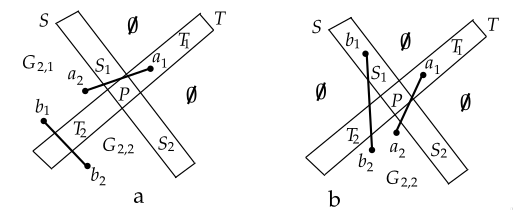
\includegraphics[width=0.5\columnwidth]{figures/3_lemma_4_case_2.png}
    \caption{Рисунок к Лемме \ref{lemma:3_4}, случай 2}
	\label{fig:3_lemma_4_case_2}
\end{figure}

Т.к. $T = T_1 \cup T_2 \cup P \cup \{b_1b_2\}$ и $|T| = k$, то 

\begin{align}
	|T_2 \cup P| &\leqslant \frac k 2 - 1 \quad \text{ тогда,  } \nonumber \\
	|R_{2, 1}| + |R_{2, 2}| &\leqslant |S| + 2 \left|T_2 \cup P \cup \{b_1b_2\}\right| \leqslant 2k \label{equation:lemma_3_4_sizes_r}
\end{align}

Напомним, что ребро $a_1a_2$ входит в множество $S$ и учтется при добавлении размера $|S|$.

Если в $\eqref{equation:lemma_3_4_sizes_r}$ достигается равенство, то ребро  $b_1b_2$ входит и в $R_{2,1}$ и в  $R_{2, 2}$.
Кроме того, каждый элемент разреза  $S$(в том числе ребро $a_1a_2$) входит в одно из множеств $R_{2,1}$ и  $R_{2,2}$

Опять рассмотрим два случая:
пусть $\Int(G_{2,1}) = \varnothing$(рисунок b).
Тогда из нормальности $T$ следует что  $\Int(H_1) = |S_1| \geqslant \frac k 2$, а следовательно $|S_2 \cup P| \leqslant \frac{k}{2} - 1$ 

Значит

 \[
	 |R_{2,2}| \leqslant |S_2| + |T_2| + |P| + |\{a_1a_2, b_1b_2\}| \leqslant k
\] 

Если и $\Int(G_{2,2}) = \varnothing$, то  $\Int(F_2) = S_2$, что противоречит нормальности разреза $T$.

Значит,  $\Int(G_{2,2}) \neq \varnothing$, но это возможно только при  $|R_{2,2}| = k$, что, в частности, означает что  $R_{2,2} \supset \{a_1a_2, b_1b_2\}$.
Тогда разрез $R_{2,2}$ нам подходит.

Иначе: $\Int(G_{2,1}) \neq \varnothing$ и  $\Int(G_{2,2}) \neq \varnothing$(рисунок a)

Тогда  $k \leqslant |R_{2,1}|$ и  $k \leqslant |R_{2,2}|$.

Следовательно, в \eqref{equation:lemma_3_4_sizes_r} достигается равенство, а значит,  $|R_{2,1}| = |R_{2,2}| = k$.
Оба разреза  $R_{2,1}$ и  $R_{2,2}$ содержат ребро  $b_1b_2$ и $a_1a_2 \in R_{2,1} \cup R_{2,2}$.
Следовательно, один из разрезов содержит оба ребра $b_1b_2$ и $a_1a_2$, а значит он удовлетворяет условиям леммы.

	\end{enumerate}

\end{proof}

\begin{customlm}{3.5} \label{lemma:3_5}
	Пусть разрезы $S, T \in \R$ зависимы, причем  $a_1a_2 \in S$ и $b_1b_2 \in T$ - различные рёбра из $E_{k+1}$.
	И  $b_1b_2 \in R_{i,j} \colon |R_{i, j}| = k$ (фиксируем эти $i, j$).

	Тогда существует разрез $R \in \R$, удовлетворяющий следующим свойствам:

	\begin{enumerate}
		\item $b_1b_2 \in R, \ \Part(R) = \{G_{i, j}, U\}$, причем либо $U = \overline G_{i, j}$, либо  $U = \overline G_{i, j} \cup \{a\}$, где  $a$ - конец ребра  $a_1a_2$, лежащий в $G_{i, j}$
		\item  $R$ независим с  $S$ и  $T$
	\end{enumerate}

\end{customlm}

\begin{proof}
	\begin{figure}[ht]
    \centering
	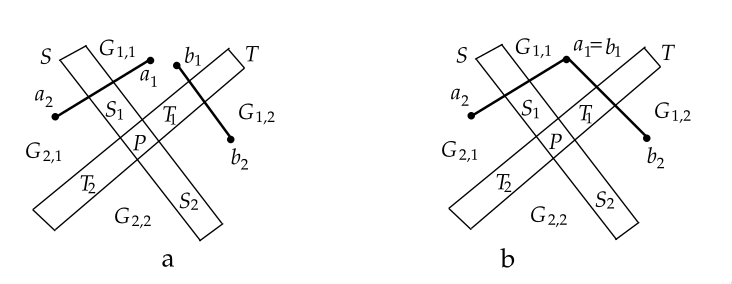
\includegraphics[width=0.5\columnwidth]{figures/3_lemma_5.png}
    \caption{Рисунок к доказательству Леммы \ref{lemma:3_5}}
	\label{fig:3_lemma_5}
	\end{figure}

Не умоляя общности $i = j = 1$. 
Т.к. $b_1b_2 \in R_{1,1}$, то один из концов ребра $b_1b_2$ лежит в $\Int(G_{1,1})$, пусть это  $b_1$.

Значит, $\Int(G_{1,1}) \neq \varnothing$ и по Лемме \ref{lemma:0_6} имеем что $R_{1,1}$ - разрез.
Более того, $\Part(R_{1,1}) = \{G_{1,1}, \overline G_{1,1}\}$.

Таким образом, при  $a_1a_2 \not \in R_{1,1}$ имеем, что $R_{1,1} \in \R$ и разрез  $R = R_{1,1}$ нам подходит.

Тогда, пусть $a_1a_2 \in R_{1,1}$.
Т.к. $a_1a_2 \in R_{1,1}$, то ребро $a_1a_2$ имеет конец в $\Int(G_{1,1})$, пусть это  $a_1$.

Рассмотрим множество $R$, полученное из  $R_{1,1}$ заменой  $a_1a_2$ на $a_1$.

Если $\Int(G_{1,1}) \neq \{a_1 \}$, то $R$ - разрез и  $\Part(R) = \{G_{1,1}, \overline G_{1,1} \cup \{a_1\}\}$(рисунок a).
Откуда очевидно следует, что этот разрез независим с $S$ и  $T$, а стало быть удовлетворяет условию леммы.

Иначе, пусть  $\Int(G_{1,1}) = \{a_1\}$(рисунок b), тогда, в частности, $a_1 = b_1$.

Кроме $a_2$ и $b_2$ эта вершина может быть смежна только с вершинами из $R_{1,1}$(т.к. внутренняя).

Тогда из $\deg_{G}(a_1) \geqslant k + 1$(это верно т.к. $a_1a_2 \in E_{k + 1}$) следует, что $|V(R_{1,1})| \geqslant k - 1$.
Но это означает, что  $|R_{1,1}| \geqslant k + 1 \implies$ противоречие.

\end{proof}

\subsection{Построение множества попарно независимых нормальных разрезов.}

\begin{customlm}{3.6} \label{lemma:3_6}
	Пусть $G$ - минимальный  $k$-связный граф, а множество  $E \subset E_{k+1}$ таково, что все разрезы из  $\R$, содержащие ребра из  $E$ - нормальные.
	Тогда существует множество  $\S = \{S_e \colon e \in S_e \}_{e \in E} \subset \R$, состоящее из попарно независимых разрезов(понятно что они также будут нормальными).
\end{customlm}

\begin{proof}
	Пронумеруем $f_1, f_2, \ldots, f_m$ ~-- ребра множества $E$.
	
	Индукция, пусть  $\S' = \{S_1, \ldots, S_{l - 1}\} \subset \R$ ~-- множество попарно независимых разрезов, причем $f_i \in S_i, \forall i < l$.

	База $|\S'| = 0$ очевидна.

	Переход: пусть $f_l \in T \in \R$, докажем, что можно изменить разрез  $T$ так, чтобы он стал независимым со всеми разрезами из  $\S'$.

	Пусть разрез  $T$ независим с разрезами  $S_1, \ldots, S_{i - 1}$, но зависим с $S_i$.
	Обозначим: $\Part(T) = \{H_1, H_2\}, \, \Part(S_i) = \{F_1, F_2\}, G_{x, y} = F_x \cap H_y$.

	Т.к. разрезы $S_i$ и  $T$ нормальны, то по Леммам \ref{lemma:3_4} и \ref{lemma:3_5} существует такой разрез  $R$, что  $f_l \in R$ и одна из частей  $R$ это  $G_{\alpha, \beta}$, а другая  либо  $\overline G_{\alpha, \beta}$ , либо  $\overline G_{\alpha, \beta} \cup \{a\}$, где $a$ - конец ребра  $f_i = ab$, лежащий в  $G_{\alpha, \beta}$.
	Обозначим эту часть как $U$.

	Хотим доказать, что $R$ независим с произвольным разрезом  $S_j, \forall j \leqslant i - 1$.

	Пусть $\Part(S_j) = \{D_1, D_2\}$. 
	Т.к. разрезы $S_i$ и  $S_j$ независимы, разрезы  $T$ и  $S_j$ также независимы, а разрезы  $T$ и  $S_i$ зависимы, то по Лемме \ref{lemma:0_7} можно считать, что $F_1 \supset D_2$, $F_2 \subset D_1$, $H_1 \supset D_2$, $H_2 \subset D_1$.

	Разберем несколько случаев:

\begin{figure}[ht]
    \centering
	\label{fig:3_lemma_6}
	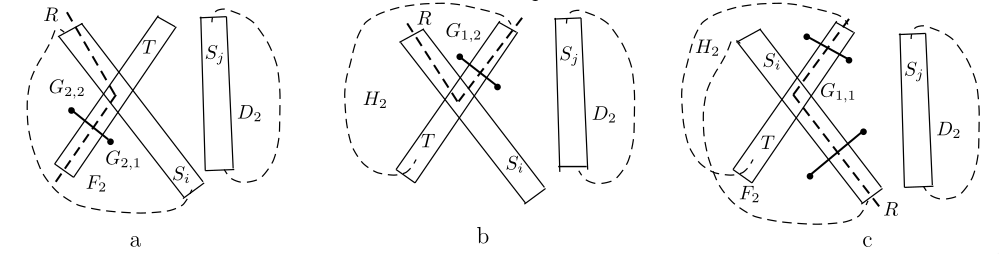
\includegraphics[width=0.7\columnwidth]{figures/3_lemma_6.png}
	\caption{Рисунок к доказательству Леммы \ref{lemma:3_6}}
\end{figure}

	\begin{enumerate}
		\item Пусть $\alpha = 2$, тогда  $G_{2, \beta} \subset F_2 \subset D_1$ и $U \supset \overline G_{2, \beta} \supset F_1 \supset D_2$(см. рис. \ref{fig:3_lemma_6} a).
			Т.е. разрезы $R$ и  $S_j$ независимы.
		\item  Пусть $\alpha = 1, \beta = 2$, тогда $G_{\alpha, \beta} = G_{1, 2} \subset H_2 \subset D_1$ и $U \supset \overline G_{1, 2} \supset H_1 \supset D_2$(см. рис. \ref{fig:3_lemma_6} b), что означает независимость разрезов $S_j$ и  $R$.
		\item  $\alpha = 1, \beta = 1$, тогда $D_1 \supset H_2 \cap F_2 = \overline G_{1, 1}$(см. рис. \ref{fig:3_lemma_6} c)ю
			Т.к. разрезы $S_i$ и  $S_j$ независимы и не имеют общих рёбер, то по Лемме \ref{lemma:0_8} получаем, что  $D_1 \supset W(S_i) \ni a$.
			А значит, $D_1 \supset \overline G_{1, 1} \cup \{a\} \supset U$.

			Из того, что $D_2 \subset F_1$ и $D_2 \subset H_1$ следует, что $D_2 \subset H_1 \setminus \Int(F_2) = G_{1, 1}$.
			Таким образом $S_j$ и  $R$ независимы.
	\end{enumerate}

\end{proof}

\subsection{Две леммы о границе разреза из $S$ (Леммы 7 и 8).}

\begin{customlm}{3.7} \label{lemma:3_7}
	Пусть $G$ ~-- минимальный  $k$-связный граф, а  $P = a_1 \ldots a_n$ ~-- простой путь, все вершины которого принадлежат множеству $V_{k + 1}$.
	Пусть существуют такие попарно независимые разрезы  $S_1, \ldots, S_{n - 1} \in \R$, что  $a_i a_{i + 1} \in S_i, \ \Part(S_i) = \{A_i, B_{i + 1}\}$, причем  $a_i \in \Int(A_i)$ и  $a_{i + 1} \in \Int(B_{i + 1})$.
	Тогда выполняются следующие утверждения:

	\begin{enumerate}
		\item $B_n \subset B_2$
		\item  $B_2 \cup \{a_1\} \supset N_G(a_n)$
	\end{enumerate}

\end{customlm}

\begin{proof}

	\begin{enumerate}
		\item  При $n = 2$ утверждение очевидно, считаем $n \geq 3$.

			Докажем, что  $B_i \supset B_{i + 1}$ при $i \in [n - 1]$.

			Т.к. разрезы  $S_{i - 1}$ и $S_i$ независимы, $a_i \in \Int(B_i)$ и $a_i a_{i + 1} \not \in S_{i - 1}$ имеем $a_{i + 1} \in B_i$(ведь иначе $S_{i - 1}$ разделяет $S$ ).


Значит, ни одна из частей $\Part(S_i)$ не может содержать $B_i \ni a_i, a_{i + 1}$(ведь $a_i, a_{i + 1}$ в разных частях  $\Part(S_i)$). В силу независимости разрезов  $S_{i - 1}, S_i$ тогда  $B_i$ содержит одну из частей $\Part(S_i) = \{A_i, B_{i + 1}\}$. 

Предположим, что $B_i \supset A_i$, см. Рис \eqref{fig:lemma_3_7}. Тогда из $a_{i - 1} \not \in B_i$ следует $a_{i - 1} \not \in A_i$.

\begin{figure}[ht]
    \centering
	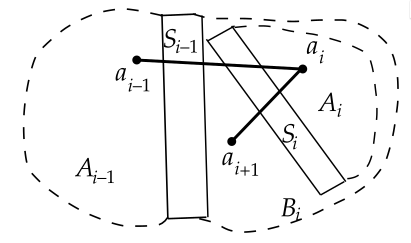
\includegraphics[width=0.4\columnwidth]{figures/lemma_3_7.png}
	\caption{Рисунок к Лемме \ref{lemma:3_7}.}
    \label{fig:lemma_3_7}
\end{figure}

Однако, вершина $a_{i - 1}$ смежна с вершиной $a_i \in \Int(A_i)$, что в силу $a_{i-1}a_i \not \in S_i$ невозможно. Следовательно, $B_i \supset B_{i + 1} \implies B_2 \supset B_n$.

\item Т.к. $a_n \in \Int(B_n)$ имеем  $N_G(a_n) \subset B_n \cup \{a_{n - 1}\}$.
	При $n = 2 \implies a_{n-  1} = a_1$, а при  $n \geqslant 3 $ у нас $a_{n - 1} \in B_{n - 1} \supset B_2 \implies N_G(a_n) \subset B_2$. 
	\end{enumerate}

\end{proof}

\begin{customlm}{3.8} \label{lemma:3_8}
	Пусть $G$ ~-- минимальный  $k$-связный граф,  $E \subset E_{k + 1}$, а множество  $\S = \{S_e \mid e \in S_e\}_{e \in E} \subset \R$ состоит из попарно независимых нормальных разрезов.
	Пусть  $R$ ~-- граница разреза  $S_e \in \S$, тогда любой простой путь с концами из  $R$ содержит ребро не из множества  $E$, для любого $e \in E$.
\end{customlm}

\begin{proof}
	От противного, рассмотрим кратчайший путь $P = a_1 a_2 \ldots a_n$ по рёбрам из $E$, такой что  $a_1, a_n \in R$.

	Если путь $P$ содержит всего одно ребро  $a_1a_2$ (т.е. $n = 2$), то $a_1a_2 \neq e$, т.к. граница $R$ содержит ровно одну вершину ребра $e \implies$. Если $n \geqslant 3$ и  $e = a_1a_2$, то перенумеруем вершины в обратном порядке и все равно добьемся того что $e \neq a_1a_2$.

	Пусть $S_i = S_{a_i a_{i + 1}}, \, \Part(S_i) = \{A_i, B_{i + 1}\}$, где  $a_i \in \Int(A_i), \; a_{i + 1} \in \Int(B_{i + 1})$.

	Т.к. разрезы  $S_e$ и  $S_1$ независимы и не имеют общего ребра, то по Лемме \ref{lemma:0_8} одна из частей $U \in \Part(S_1)$ содержит  $W(S_e)$.
	А значит  $U \supset R \ni a_1$, откуда следует  $U = A_1$.

	По Лемме \ref{lemma:3_7} следует, что  $N_G(a_n) \subset B_2 \cup \{a_1\}$, см. Рис. \eqref{fig:lemma_3_8}.
\begin{figure}[ht]
    \centering
	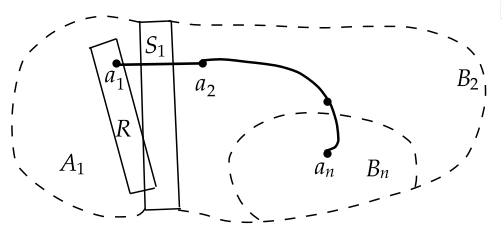
\includegraphics[width=0.4\columnwidth]{figures/lemma_3_8.png}
	\caption{Рисунок к Лемме \ref{lemma:3_8}.}
    \label{fig:lemma_3_8}
\end{figure}

Т.к. разрез $S_e$ нормален, $\Int(A_1) \neq \{a_1\}$ \todo{почему?} (ведь $S_1$ тоже нормальный, работает при $k \geqslant 4$), то $R \in \R_k(G)$ \todo{почему?}.

Из $R \subset A_1 \implies R$ не разделяет  $B_2 \cup W(S_1)$.
Значит, одна из компонент связности $M$ графа $G - R$ лежит в $\Int(A_1) \setminus \{a_1\}$(ведь компонент связности у $G - R$ хотя бы две и одна целиком содержит  $B_2 \cup W(S_1)$).
Из $k$-связности графа  $G$ следует, что вершина $a_n \in R$ должна иметь смежную вершину в  $M \subset \Int(A_1)$, что противоречит тому что $N_G(a_n) \subset B_2 \cup \{a_1\}$.
\end{proof}

\subsection{Лемма о кривых разрезах.}

\begin{customlm}{3.9} \label{lemma:3_9}
	Пусть $G$ ~-- минимальный  $k$-связный граф, причем в множестве  $\R$ есть кривые разрезы.
	Тогда  $e_k + c \geqslant k + 1$.
\end{customlm}

Обозначения смотреть в \ref{prop:for_minimum_k_connected_graph}.

Доказательство напишем дальше, везде через $S_e$ обозначаем разрез из $\R$, содержащий ребро $e \in E_{k + 1}$.

Понятно, что при  $k = 2$ кривых разрезов не существует(ведь внутренность каждой части по одному разрезу не пуста).
Поэтому везде далее считаем  $k \geqslant 3$.

\begin{customclaim}{1} \label{claim:3_1}
	Пусть $a_1a_2 \in E_{k + 1}$, разрез $S_{a_1 a_2}$ ~-- кривой, причем $a_1 \in A_1 \in \Part(S_{a_1a_2})$ и $|\Int(A_1)| < \frac{k}{2}$.

	Тогда выполнено следующее:

	\begin{enumerate}
		\item Существует ребро $aa' \in E_{k + 1} \colon a$ ~-- висячая вершина  $G_{k + 1}$ и разрез  $S_{aa'} \in \R$ ~-- кривой. Более того, если $a \in A \in \Part(S_{aa'})$, то  $|\Int(A)| < \frac{k}{2}$.

		\item Пусть $\deg_{G_{k + 1}}(a_1) > 1, \; a$ ~-- такой лист леса $G_{k + 1}$, что путь по  $G_{k + 1}$ из $a_1$ в $a$ не проходит через $a_2$, а $a'a$  ~-- последнее ребро этого пути. Тогда ребро  $aa'$ подходит для пункта 1.
	\end{enumerate}

\end{customclaim}

\todo[inline]{чтобы использовать утв1 в лемме 9, нам ведь надо чтобы существовал какой то кривой разрез над ребром из $E_{k+1}$, как мы говорим что такой есть?}

На рисунках квадратиком обозначены вершины степени $= k$, а кружочками вершины степени  $> k$.

\todo[inline]{ниже}

{\color{red} пусть мы рассматриваем разрез $S_{ab}$ по ребру $ab$, правда ли что тогда  $a, b$ обязаны быть смежны со всеми вершинами  $S_{ab}$?

Т.е. мы удалили ребро и граф перестал быть $k$ связным, это значит что  $a, b \not \in S_{ab}$, ведь тогда исходгный граф не был бы $k$-связным. Значит что после удаления $k - 1$ и ребра  $ab$ граф не свяезн, а если удалить просто  $k - 1$ вершину, что граф связен. Значит что это ребро соединяет обе компоненты. И обратно, вернуть любую вершину из $S_{ab}$, то граф опять станет связным. Ну чето вроде может быть так что}

% \todo[inline]{пусть мы рассматриваем разрез $S_{ab}$ по ребру $ab$, правда ли что тогда  $a, b$ обязаны быть смежны со всеми вершинами  $S_{ab}$?

%  }

\begin{proof}[\normalfont\textsc{Доказательство Леммы \ref{lemma:3_9}}]
	Пусть $a_1$ ~-- лист в $G_{k + 1}$ и при этом $|\Int(A_1)| = p < \frac{k}{2}, S = V(S_{a_1a_2})$, где $a_2$ ~-- сосед $a_1$ в $G_{k + 1}$.
	Такой лист существует по Утверждению \ref{claim:3_1}.

	Пусть $M = \Int(A_1) \cap V_k, \; m = |M|$. Смотреть Рис. \eqref{fig:lemma_3_9_a}.

\begin{figure}[ht]
    \centering
	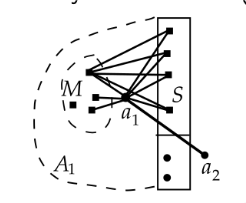
\includegraphics[width=0.25\columnwidth]{figures/lemma_3_9_a.png}
	\caption{Рисунок к Лемме \ref{lemma:3_9}, случай a.}
    \label{fig:lemma_3_9_a}
\end{figure}

Вершина $a_1$ не может быть смежна с вершинами из $V_{k + 1} \cap A_1$, т.к. является листом в $G_{k + 1}$.

Следовательно, вершина $a_1$ смежна не более чем с $m$ вершинами из $\Int(A_1)$.

Т.к. $\deg_G(a_1) \geqslant k + 1$, $a_1$ смежна только с вершинами из $\Int(A_1), S$, то $a_1$ несмежна с не более чем $m - 1$ вершинами из  $S$.

Все смежные с $a_1$ вершины из $S$ имеют степень $k$.

Имеем:
\begin{align*}
	|\Int(A_1) \cap V_{k + 1}| &= p - m \\ 
	|S \cap V _{k + 1}| &\leqslant m - 1 \implies \\
	|A_1 \cap V_{k + 1}| &= |\Int(A_1) \cap V_{k + 1}| + |S \cap V_{k + 1}| \leqslant p - 1
\end{align*}

Случай 1. $m \geqslant 2$. Как в слайдах.

Случай 2.  $m = 1$.

....

{\color{blue}$T'$ является лесом, т.к. это целые компоненты связности исходного дерева  $T$, ведь ребер во вне идти не может, а с $a_1$ они не соединены по построению.}


\begin{figure}[ht]
    \centering
	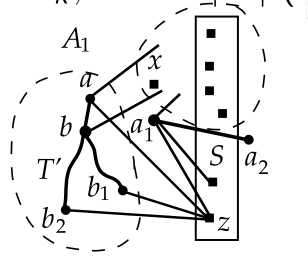
\includegraphics[width=0.25\columnwidth]{figures/lemma_3_9_b.png}
	\caption{Рисунок к Лемме \ref{lemma:3_9}, случай b.}
    \label{fig:lemma_3_9_b}
\end{figure}

Возьмем произвольное $a \in Y, \deg_{T'}(a) \leqslant 1$, тогда т.к. $\deg_G(a) \geqslant k + 1$ и в $A_1$ у нас всего $k$ вершин степени  $k$, следует, что  $a$ смежна с одной вершиной $V_{k + 1}$ и $k$ вершинами из  $V_{k}$, т.е. $\deg_{T'}(a) = 1$.
Причем $a$ обязана быть смежна с  $x$ и со всеми  $k - 1$ вершинами  $S$.
Таким образом, лес  $T'$ не содержит изолированных вершин и состоит из одной компоненты.

...

Рассмотрим разрез $S_{ab} \in \R$, вершина $b$ смежна хотя бы с $k - l + 1$ вершинами множества  $S \cup \{x\}$. 
И при $b$ смежна со всеми вершинами  $S_{ab}$, но т.к. $|S_{ab}| = k - 1, \, k - l + 1 \geqslant k$, то $b$ смежна и с вершиной вне  $S_{ab}$.
\todo[inline]{и что? почему все из $S \cup \{x\} \cup \N_G(b)$ обязаны лежать в $S_{ab}$?}
 

\end{proof}

\subsection{Множество попарно независимых разрезов: cвойства крайних частей (леммы 10-13). Теорема Мадера о количестве вершин степени k в минимальном k-связном графе.}


\begin{proof}[\normalfont\textsc{Доказательство Леммы 10}]
	в первом пункте, имеет $v_k \geqslant k + 1$, т.к. каждая вершина  $V_{k + 1}$ смежна только с вершинами из $V_k$. Случай  $v_{k + 1} = 0$ тривиален.
\end{proof}

\begin{proof}[\normalfont\textsc{Доказательство Леммы 12}]
	Внутри $B_i$ найдется вершина степени  $k$, т.к.  $a_{i}$ имеет степень $k + 1$, может быть смежна только с  $k$ вершинами из $|R_i|$, а значит смежна с какой то вершиной внутри  $B_i$, как мы поняли все вершины внуртри  $A_i$ степени  $k + 1$ изолированны в  $G_{k + 1}$, значит сосед $a_{i}$ внутри $B_i$ степени $k$.
\end{proof}

\begin{proof}[\normalfont\textsc{Доказательство Леммы 13}]
	"По Лемме 8...", подробнее: $p_1$ это количество вершин степени $k$ в  $R_1$, значит в нем $k - p_1$ вершин степени $> k$. У нас все разрезы нормальные и тогда по Лемме \ref{lemma:3_8} получаем что не будет пути между двумя вершинами степени  $k + 1$, значит они в разных компонентах.

	При  $p_1 = 0$ у нас $c \geqslant k$.
\end{proof}
\subsection{Если граф $G$ — минимальный $k$-связный, то граф $G'$ (полученный отрезанием графа $K_{k,k}$ от крайней части и заменой его на новую вершину степени $k$) — тоже (утверждения 3 и 4).}

\subsection{Доказательство теоремы о виде минимальных $k$-связных графов с минимальным числом вершин степени $k$ (без утверждений 3 и 4).}

надо доказать теорему 2, утверждения 1, 2 в том числе. начиная со слайда "Доказательство Теоремы 2."

\begin{proof}[\normalfont\textsc{Доказательство Утверждения 2}]
	Чтобы показать что $x \in S_{y_1y_2}$, я бы сказал, что пользуясь леммой 7 у нас $Y_2 \supset Y_3 \dots \supset Y_m \ni y_m$ и при этом $x$ смежен  $y_1, y_m$, а они во внутренностях. Ну вот и получили.(хотя почему $y_m \in \Int(y_2)$?).

	После этого говорим что можно взять две крайних части  $A_i, A_j$, у которых границы содержат по вершине каждого дерева и проследить путь по этим вершинам. Тогда будет  $k$ независимых пересечений разреза  $S_{y_1 y_2}$, а значит нет месте вершине $x$ внутри разреза  $S_{y_1y_2}$.
\end{proof}

\subsection{Алгоритм построения минимальных $k$-связных графов с минимальным числом вершин степени $k$.}

\subsection{Минимальные графы связности не более 5: расцепление хорошей и плохой пары зависимых разрезов.}

\begin{proof}[\normalfont\textsc{Доказательство Леммы 14}]
	Не только по Лемме \ref{lemma:3_2}, а скорее аналогично док-ву Леммы \ref{lemma:3_4}.
\end{proof}

\begin{proof}[\normalfont\textsc{Доказательство Леммы 15}]
	"В этом случае $|R_{2, 1}| \geq k$ и $|R_{2, 2}| \geq k$" -> т.к. внутренности их частей не пусты.

	"Пусть вершины $b_1$ и $a_1$ несмежны. Так как $d_G(b_1) \geq k + 1$, а все вершины, смежные с $b_1$ лежат в $S_1 \cup (V(T) \cup \{b_2\})$" -> у нас в $S_1$ лежит $b_1$, а еще знаем что хотя бы одна вершина(а именно $a_1$) не смежна с $b_1$ и лежит в $T$, а значит  $S_1 \cup (V(T) \cup \{b_2\}) \leqslant |S_1| + (k - 2) + 1 = |S_1| + k - 1$, значит $|S_1| > 3$, ведь  $b_1$ себе не сосед.
\end{proof}

\subsection{Минимальные графы связности не более 5: построение множества попарно независимых разрезов.}

\subsection{Теорема Халина о цикле минимального трёхсвязного графа.}

смотреть два рисунка

\begin{figure}[ht]
    \centering
	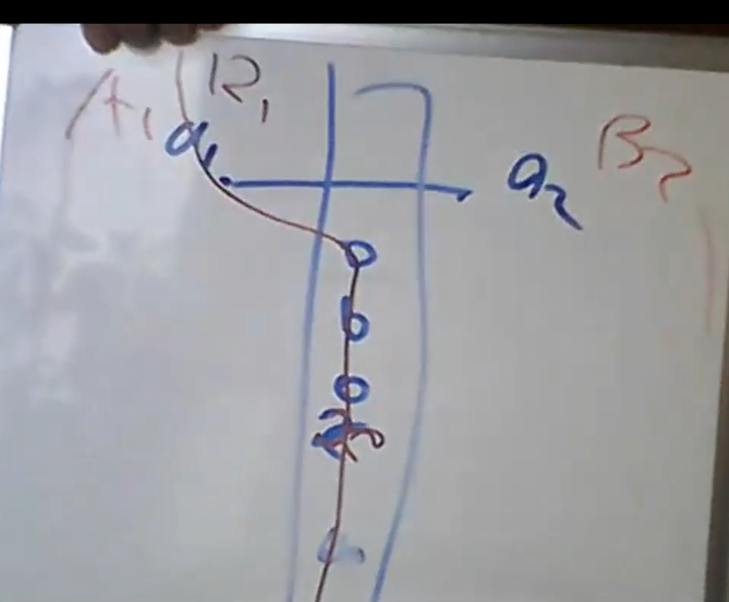
\includegraphics[width=0.4\columnwidth]{figures/theorem_3_4.png}
    \caption{Рисунок 1 к Теореме 3}
\end{figure}

\begin{figure}[ht]
    \centering
	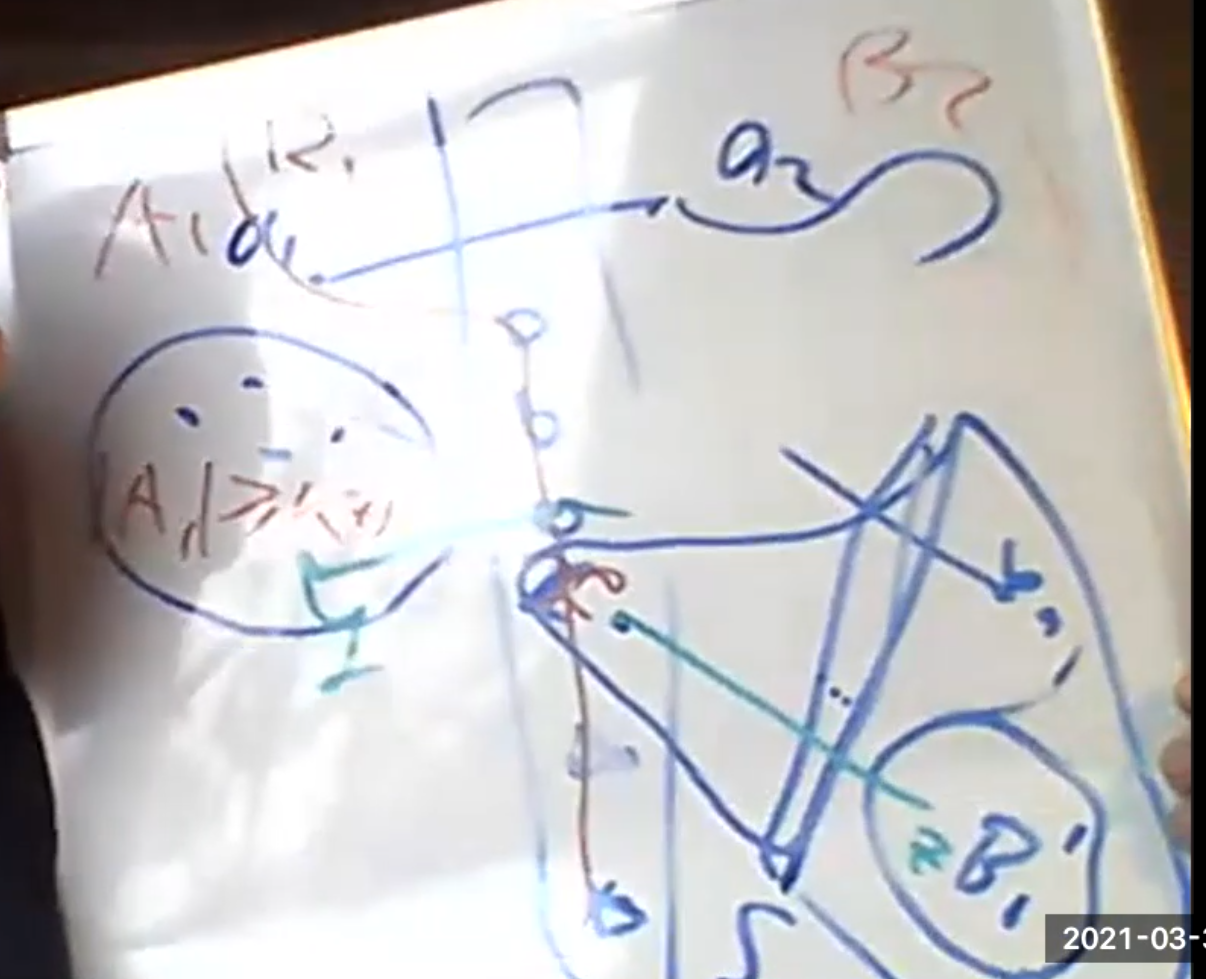
\includegraphics[width=0.4\columnwidth]{figures/theorem_3_4_2.png}
    \caption{Рисунок 2 к Теореме 3}
\end{figure}
